\documentclass[11pt]{article}
\usepackage[a4paper,margin=0.65in]{geometry}
\usepackage[T1]{fontenc}
\usepackage{lmodern}
\usepackage{tikz}
\usetikzlibrary{arrows.meta,positioning,shapes.geometric,fit,calc}
\usepackage{pdflscape}
\usepackage{float}
\usepackage{caption}
\pagestyle{plain}
\setlength{\parindent}{0pt}

\tikzset{
  classbox/.style={draw, rounded corners=2pt, fill=blue!3, align=left,
    font=\small, inner sep=5pt, text width=5.0cm},
  smallclass/.style={draw, rounded corners=2pt, fill=blue!3, align=left,
    font=\small, inner sep=5pt, text width=4.2cm},
  module/.style={draw, rounded corners=3pt, fill=teal!7, align=center,
    minimum height=9mm, text width=3.4cm, font=\small},
  datastore/.style={draw, cylinder, shape border rotate=90, aspect=0.25,
    fill=orange!10, align=center, minimum height=9mm, text width=2.8cm, font=\small},
  decision/.style={diamond, draw, fill=yellow!12, align=center, aspect=2.0,
    inner sep=2pt, font=\small},
  flow/.style={-{Stealth[length=2.2mm]}, thick},
  dependency/.style={-{Stealth[length=2mm]}, dashed, thick},
  association/.style={-{Stealth[length=2mm]}, thick}
}
\begin{document}
\begin{center}
{\LARGE\bfseries Automated Plagiarism Checker}\\[2mm]
{\large Overall Program Workflow Flowchart}
\end{center}
\vspace{4mm}

\begin{figure}[H]\centering
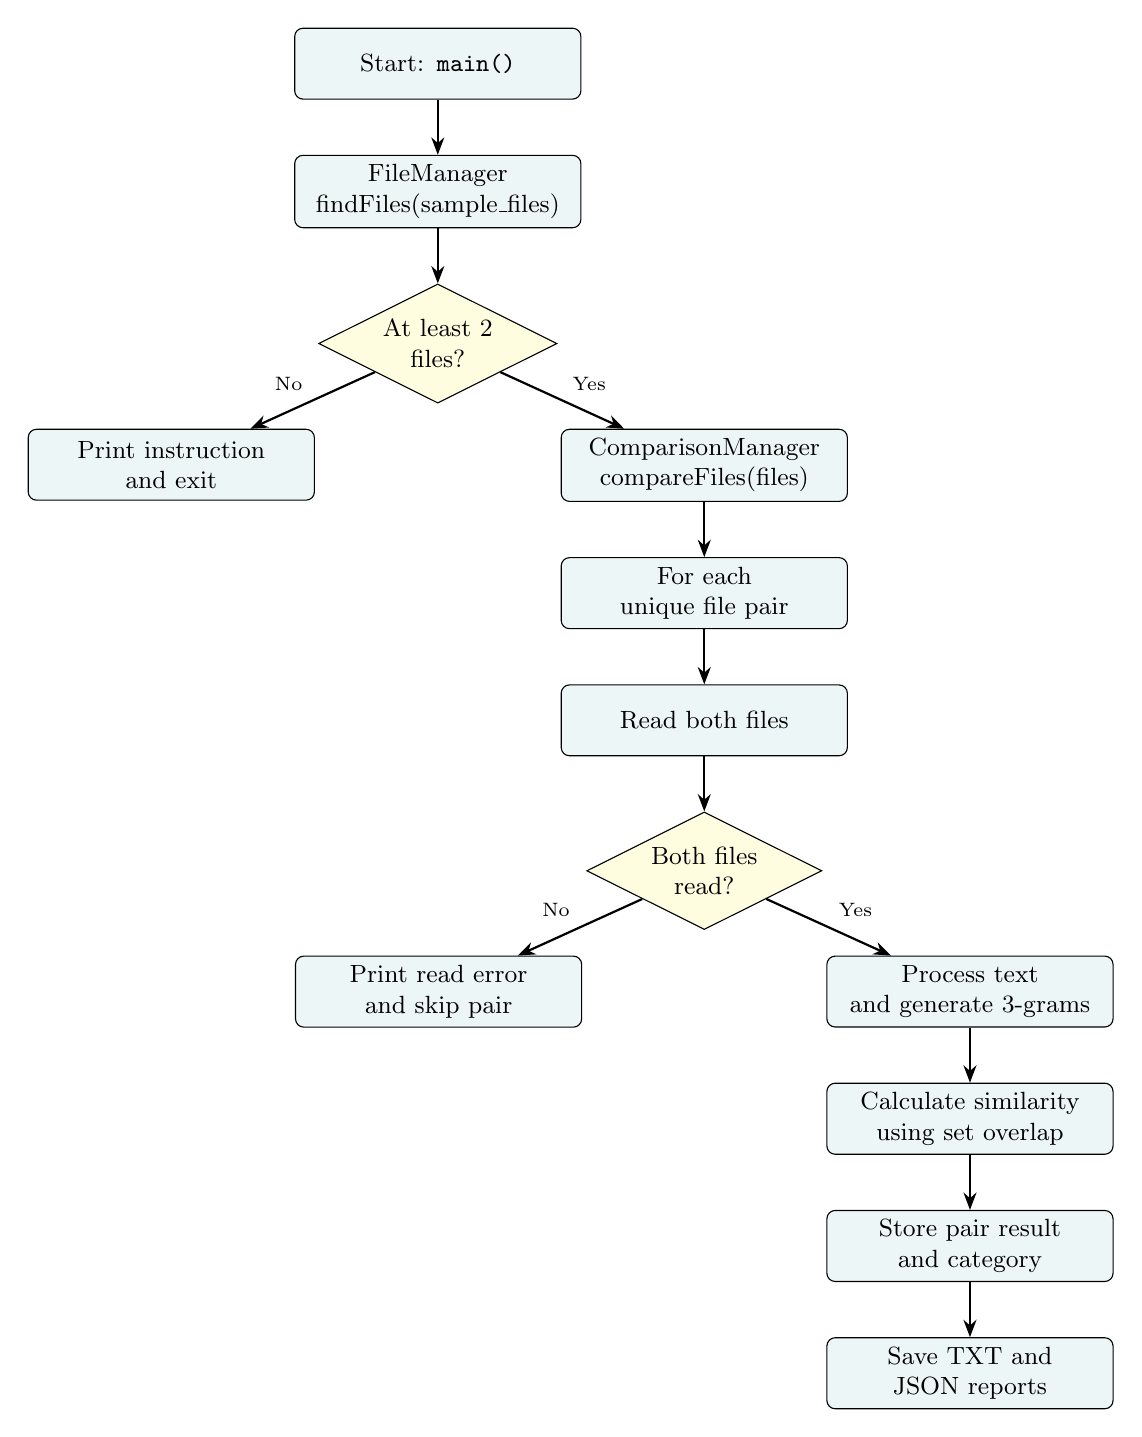
\begin{tikzpicture}[node distance=7mm and 8mm]
\node[module] (start) {Start: \texttt{main()}};
\node[module,below=of start] (discover) {FileManager\\findFiles(sample\_files)};
\node[decision,below=of discover] (enough) {At least 2\\files?};
\node[module,below left=of enough] (stop) {Print instruction\\and exit};
\node[module,below right=of enough] (compare) {ComparisonManager\\compareFiles(files)};
\node[module,below=of compare] (pair) {For each unique file pair};
\node[module,below=of pair] (read) {Read both files};
\node[decision,below=of read] (readok) {Both files\\read?};
\node[module,below left=of readok] (skip) {Print read error\\and skip pair};
\node[module,below right=of readok] (process) {Process text\\and generate 3-grams};
\node[module,below=of process] (sim) {Calculate similarity\\using set overlap};
\node[module,below=of sim] (result) {Store pair result\\and category};
\node[module,below=of result] (save) {Save TXT and JSON reports};
\draw[flow] (start)--(discover);
\draw[flow] (discover)--(enough);
\draw[flow] (enough)--node[above left,font=\scriptsize]{No}(stop);
\draw[flow] (enough)--node[above right,font=\scriptsize]{Yes}(compare);
\draw[flow] (compare)--(pair);
\draw[flow] (pair)--(read);
\draw[flow] (read)--(readok);
\draw[flow] (readok)--node[above left,font=\scriptsize]{No}(skip);
\draw[flow] (readok)--node[above right,font=\scriptsize]{Yes}(process);
\draw[flow] (process)--(sim);
\draw[flow] (sim)--(result);
\draw[flow] (result)--(save);
\end{tikzpicture}
\caption{Actual console workflow implemented in main.cpp and ComparisonManager.cpp.}
\end{figure}

\end{document}
